\documentclass[a4paper,12pt]{article}
\usepackage{color}
\usepackage{amsmath} % do fancy math
\usepackage{mathtools}
\usepackage{amsfonts}
\usepackage{bm}
\usepackage{amsthm} % math theorem proof etc
\usepackage{graphicx} % import images
\usepackage{tikz} % draw images with latex
%\usetikzlibrary{arrows,decorations.pathmorphing,backgrounds,positioning,fit,petri}
\usepackage{pgf} % go with tikz
\usepackage{subfigure}
\usepackage{caption}
%\usepackage{subcaption}
\usepackage{multirow}
\usepackage{algorithm}
\usepackage{algorithmic}
\usepackage{epstopdf}
\usepackage[round]{natbib}
\usepackage{setspace}
\usepackage[top=30mm, bottom=30mm, left=35mm,right=30mm]{geometry}
\newcommand{\ud}{\,\mathrm{d}}
\newcommand{\vx}{\mathbf{x}}
\newtheorem{defi}{Definition}[section]
\newtheorem{theorem}{Theorem}[section]
\newtheorem{lemma}[theorem]{Lemma}
%------------Y(^_^) I'm the happy separation line (^_^)Y-------------%


%------------Y(^_^) I'm the toolbox for lazybones (^_^)Y-------------%
% Maths
% \begin{equation*}
%
% \end{equation*}
% \mathcal{}
% \!  \,  \:  \;

% Graph
% \begin{figure}[htbp]
% \begin{center}
% \includegraphics[scale=1.1,trim=2cm 0cm 0cm 2cm]{name.pdf}
% \end{center}
% \caption[short]{long}
% \label{fig:3.2}
% \end{figure}

% Fonts
% \textbf{} \textsf{} \textit{} \textt{}

% Paragraph
% \onehalfspacing  \doublespacing
% setlength{\parindent}{0in}

% title
% \title{}
% \author{Zhe Sha}
% \date{1-Jan-1111}
% \maketitle

%------------Y(^_^) I'm the toolbox for lazybones (^_^)Y-------------%
\begin{document}

\title{Experiment 1a}
\author{Zhe Sha}
\maketitle

\onehalfspacing
\numberwithin{equation}{section}
%------------Y(^_^) I'm the happy separation line (^_^)Y-------------%

\section{Introduction}
In this report we present results of Experiment 1a that focuses on updating a uni-variate process with single source of observations. The main purpose is to develop a complete implementation of the Bayesian hierarchical model framework on the sphere that is simple enough for debugging and tuning (model or algorithm related) parameters.

In Experiment 1a, we test on the GIA process with synthetic GPS data. Over the period of 2005 to 2015, we assume the GIA process is a time invariant spatial process that represent a yearly trend in $mm$. The GPS data are processed to reflect only the vertical movement of the earth, also in $mm/yr$. Denote the GIA process by $X_{GIA}$ and the GPS observation by $Y_{GPS}$, then the Bayesian hierarchical model can be written as
\begin{align}
\left\{\begin{array}{l}
\bm{Y}_{GPS} | \bm{X}_{GIA}, \bm{e} = \bm{A} \bm{X}_{GIA} + \bm{e} \\
\bm{X}_{GIA} | \bm{\mu}_{GIA}, \bm{Z}_{GIA} = \bm{\mu}_{GIA} + \bm{Z}_{GIA} \\
\bm{Z}_{GIA} | \rho, \sigma^2 \sim \mathcal{GP}(0, K_{\nu}(\cdot, \cdot \, | \rho, \sigma^2))
\end{array}
\right.
\end{align} 
where $A$ is the linear mapping operator from the process to the observations, $\bm{e}$ is a vector of the measurement errors of the GPS data that are assumed to be known, $\bm{\mu}_{GIA}$ is the prior GIA mean field which can usually be derived from some physical models, $\bm{Z}_{GIA}$ is a stationary zero mean Gaussian spatial process with Mat\'{e}rn covariance function, and $\rho, \sigma^2, \sigma_e^2$ are the hyper-parameters to be estimated.   

In the following, we use the ICE-6G results on one degree resolution as the prior GIA mean field. The synthetic data are generated by adding Gaussian noises to the ICE-6G data at the location of the selected GPS station. 

\section{Choosing Mesh}
Before moving on to the estimation and prediction, we need to choose a mesh grid for approximating the SPDE model by a sparse representation as an Gaussian Markov random field (GMRF). The mesh can not only affect the estimation results of the hyper parameters but also the marginal errors of the latent field. General rules of thumb for choosing a mesh grid are 
\begin{enumerate}
\item keep a few observations on the mesh grid to assess the noises;
\item avoid undesirable variabilities or sharp changes in the shape and size of the triangles;
\item tune resolutions at different locations according to the problem. e.g. Dense grid at observations or area of interest and sparse else where with a smooth change of the resolution at the boundaries.
\end{enumerate}

The R packages \textbf{INLA} provides functions for generating meshes on the sphere, either by building up from starting locations or by sub-dividing the globe in to semi-regular grid. 
\begin{verbatim}
R> mesh1 <- inla.mesh.2d(loc = my_loc, cutoff = 0.05,  max.edge = 0.1)
R> mesh2 <- inla.mesh.create(globe = 10)
\end{verbatim}
The resolutions can be controlled by \texttt{max.edge}, the maximum edge length of the triangles, or \texttt{globe} the number of sub-segments. We can also set a cut-off value \texttt{cutoff} such that points with distance smaller than the cut-off values are considered to be the same and thus avoiding dramatic change of the triangle size.

The locations need to be represented by 3D Cartesian coordinates and with a commonly used ``longlat'' coordinates, the converting can be done by 
\begin{verbatim}
R> loc_Cart <- inla.mesh.map(loc_longlat, projection = "longlat")
\end{verbatim} 

Below we illustrate the effect of meshes by two examples. In the first example, we use three different strategies to generate the mesh with different resolutions and compare the marginal standard errors of the latent field given by these meshes. In the second experiment, we compare the estimation and prediction results from a set of meshes.

\subsection{Comparing marginal standard errors}
The three strategies to generate the meshes are
\begin{enumerate}
\item use the regular grid of GIA locations as initial mesh locations;
\item use the GPS location which are irregular as initial mesh locations;
\item use a semi-regular mesh on the globe which subdivides a icosaheron by a given number of sub-segments to use.
\end{enumerate}

For each strategy, we generate three meshes with resolution from low to high by tuning the corresponding parameters. In producing the marginal standard error, we fix the hyper parameters in the SPDE model to some prior values, say $\kappa = 80.59$ and $\tau = 0.00039$ which correspond to a range\footnote{Transformation between the hyper-parameter space and the setting of the prior will be discussed in the Section \ref{sec:hyperpar}} $\rho = 0.0785$ (about $500km$) and variance $\sigma^2 = 20^2$.

First we generate the mesh by using the GIA locations. The GIA locations are on a grid of 1 degree resolution. When project back to the globe, the grid become much denser at the polar areas. To generate a mesh with triangles of similar size, we set cut-off and maximum edge distances as multiples the minimum distance of two points lying on the grid line nearest to the equator (in this case 0.5 or -0.5). Below shows the code for generating the meshes.
\begin{verbatim}
Mesh_GIAs[[1]] <- inla.mesh.2d(loc = GIA_loc6, cutoff = u_dist*8, 
                               max.edge = u_dist*12) 
Mesh_GIAs[[2]] <- inla.mesh.2d(loc = GIA_loc6, cutoff = u_dist*3, 
                               max.edge = u_dist*6) 
Mesh_GIAs[[3]] <- inla.mesh.2d(loc = GIA_loc6, cutoff = u_dist, 
                               max.edge = u_dist*3)
\end{verbatim}

Table \ref{tab:GIA_mesh} below shows summary of the meshes.

\begin{table}[htbp] 
\centering
\caption{Summary of meshes generated by GIA locations}\label{tab:GIA_mesh}
\begin{tabular}{ c| c c }
\hline
 Mesh     & Vertices & Triangles \\\hline
 Small  &  646 & 1288 \\ 
 Medium & 4043 & 8082 \\  
 Large  & 26614 & 53224 \\   \hline
\end{tabular}
\end{table}

Figure \ref{fig:GIA_mesh} shows the marginal standard deviations of the latent field by using three meshes generated by the GIA locations. The patterns and the bands in the plots are purely caused by the triangulations. Apparently, we do want avoid such effects so regular longlat projected grid are not desirable in producing the mesh.
\begin{figure}[htbp]
 \begin{center}
 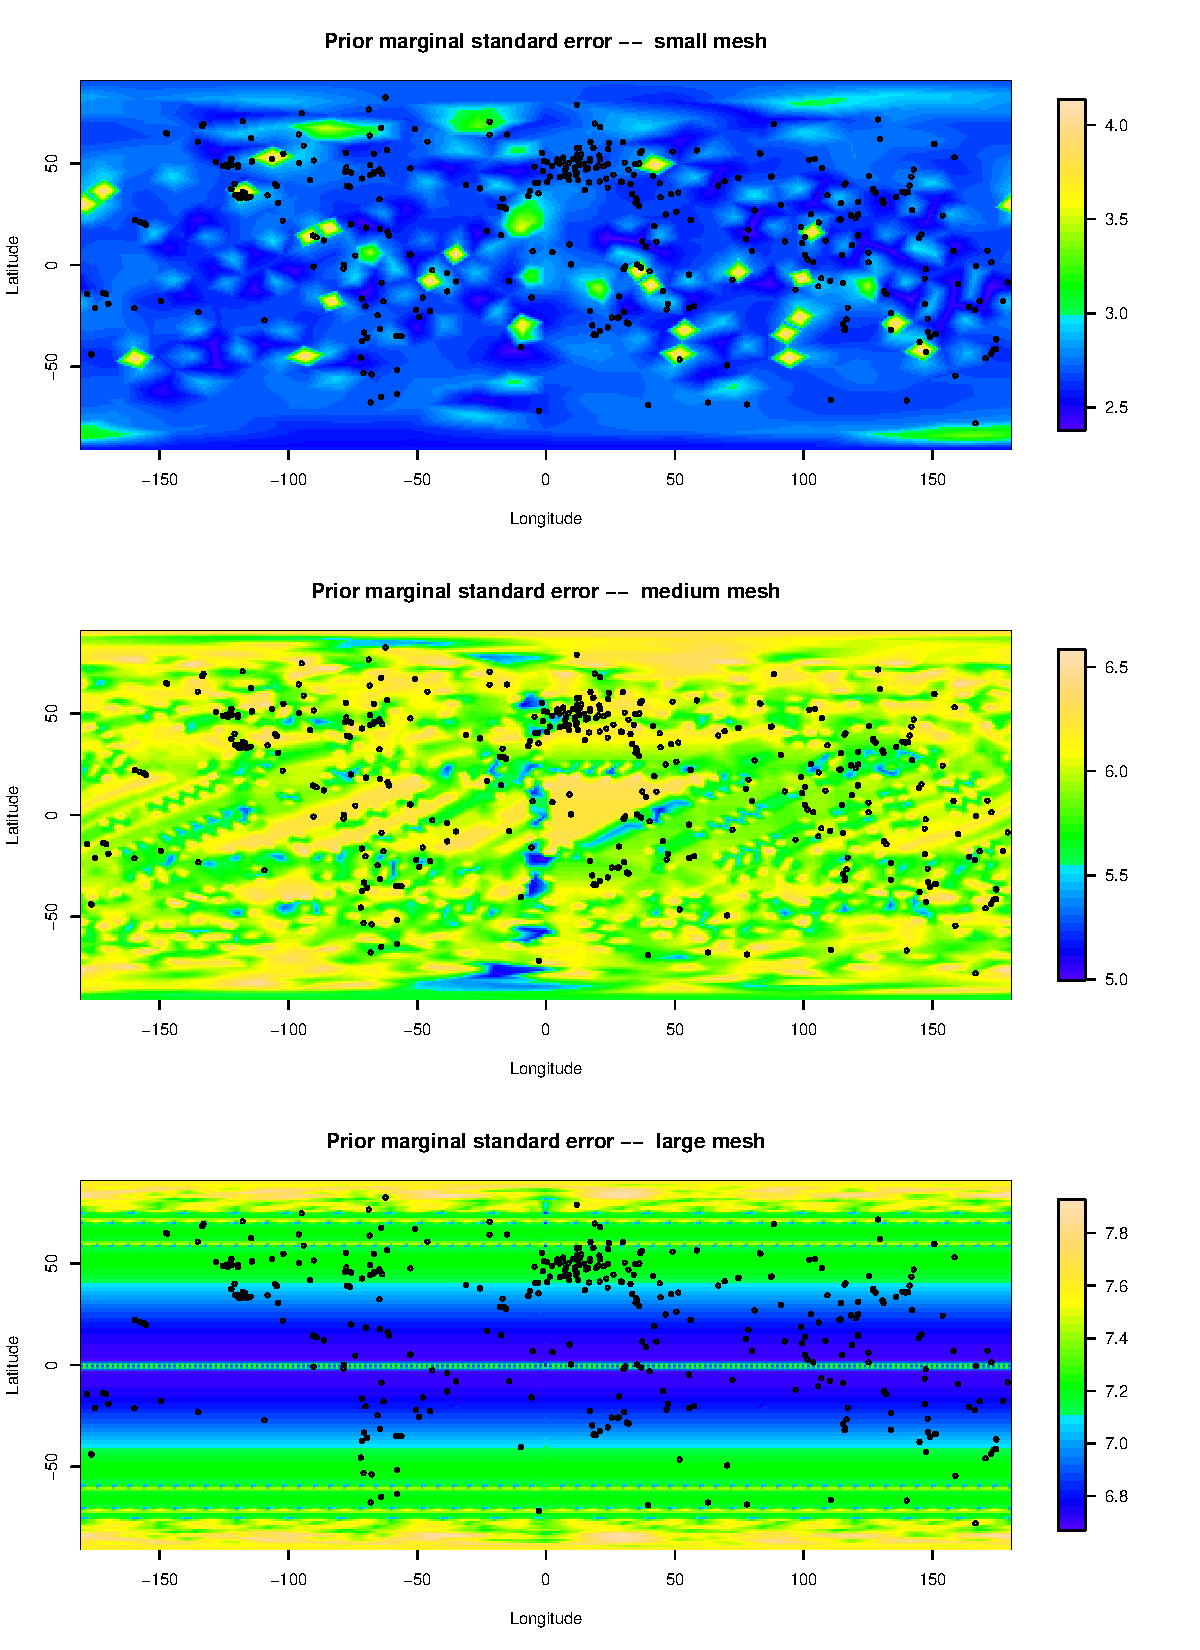
\includegraphics[scale=0.8]{fig/prior_GIAmesh.pdf}
 \end{center}
 \caption[GIA mesh]{Marginal standard deviations of the latent field given by meshes generated by GIA locations. The mesh get denser from top to bottom.}
 \label{fig:GIA_mesh}
 \end{figure} 
 
Next we show the results by using GPS locations. Similarly we use the same cut-off and maximum edge unit. The summary is included in Table \ref{tab:GPS_mesh} and Figure \ref{fig:GPS_mesh}
\begin{verbatim}
mesh_GPS[[1]] <- inla.mesh.2d(loc = GPS_loc, cutoff = u_dist*5,  
                              max.edge = u_dist*12)
mesh_GPS[[2]] <- inla.mesh.2d(loc = GPS_loc, cutoff = u_dist*3,
                              max.edge = u_dist*5)
mesh_GPS[[3]] <- inla.mesh.2d(loc = GPS_loc, cutoff = u_dist/3, 
                              max.edge = u_dist*2)
\end{verbatim} 

\begin{table}[htbp] 
\centering
\caption{Summary of meshes generated by GPS locations}\label{tab:GPS_mesh}
\begin{tabular}{ c| c c }
\hline
 Mesh     & Vertices & Triangles \\\hline
 Small  &  735 & 1466 \\ 
 Medium & 4099 & 8194 \\  
 Large  & 25694 & 51384 \\   \hline
\end{tabular}
\end{table}

\begin{figure}[htbp]
 \begin{center}
 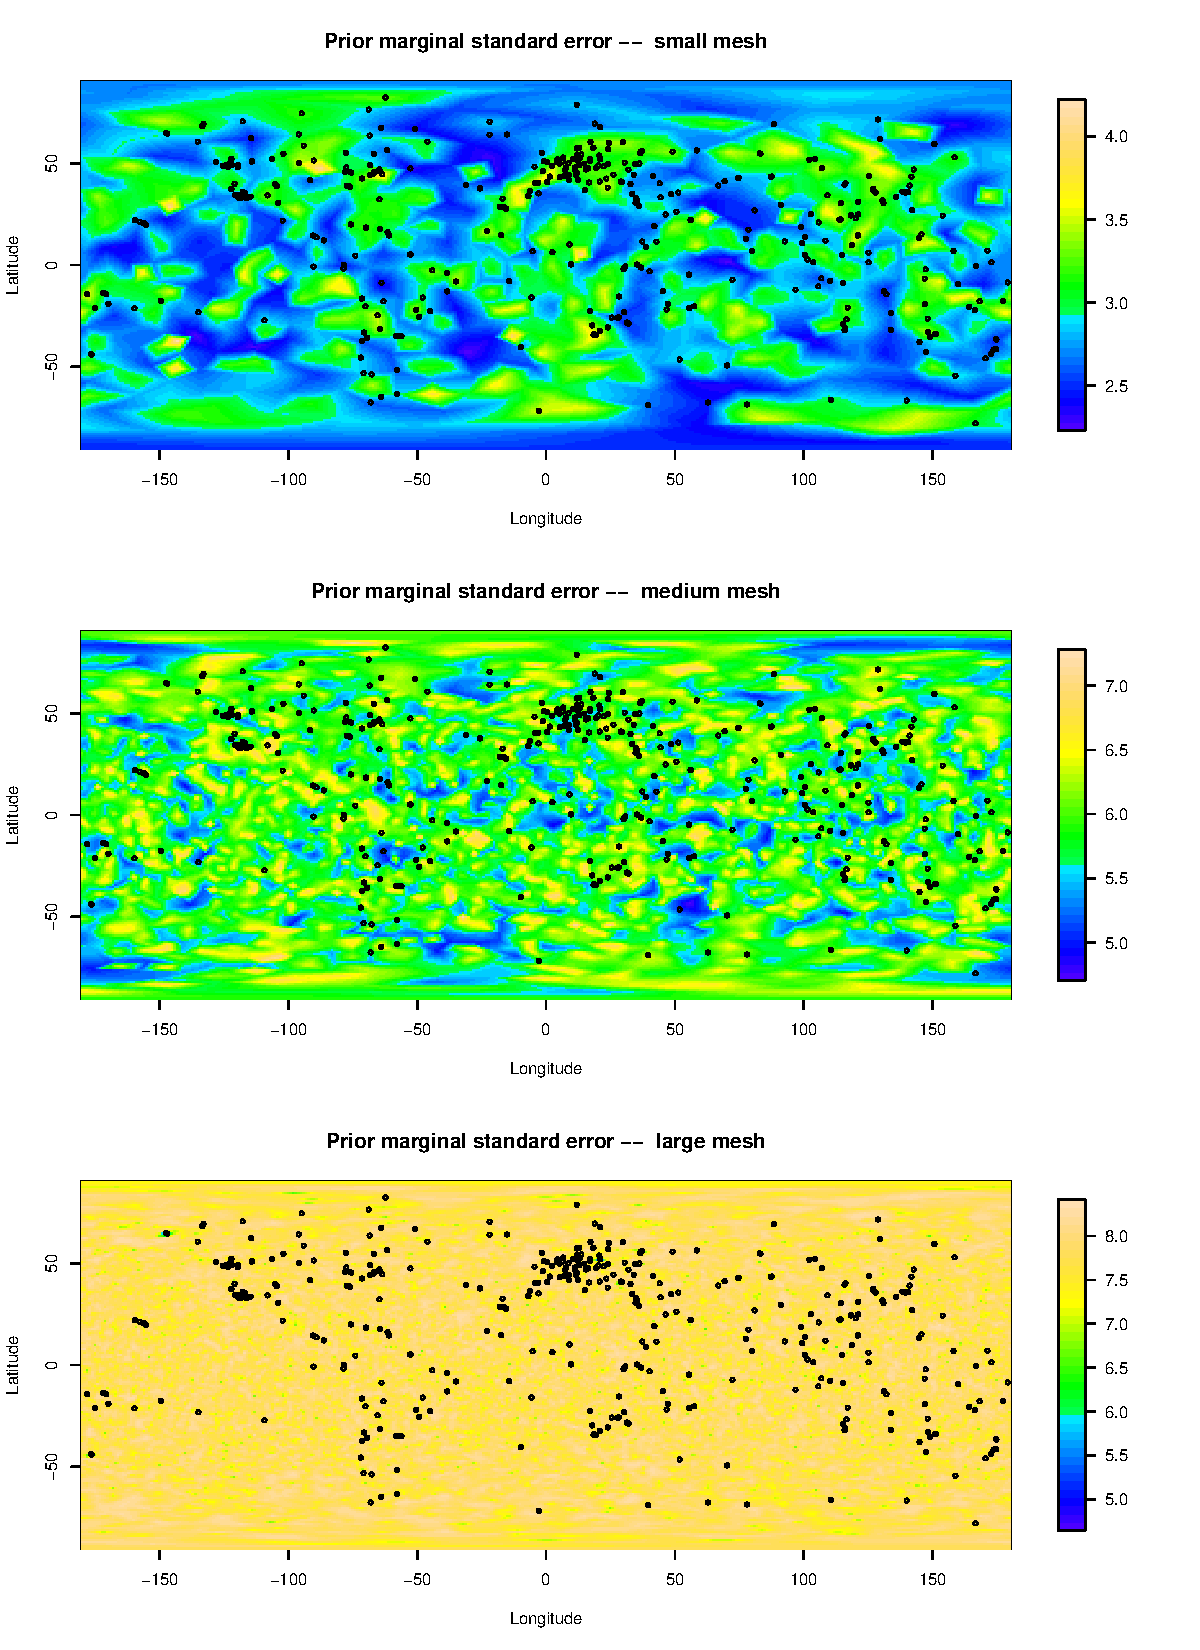
\includegraphics[scale=0.8]{fig/prior_GPSmesh.pdf}
 \end{center}
 \caption[GPS mesh]{Marginal standard deviations of the latent field given by meshes generated by GPS locations. The mesh get denser from top to bottom.}
 \label{fig:GPS_mesh}
 \end{figure}

The plots show less pattern compared to the GIA ones as the GPS locations are irregular. The large mesh looks desirable as the standard deviations are almost homogeneous.

Finally we show the results of a semi-regular mesh on the globe.
\begin{verbatim}
mesh_regs[[1]] <- inla.mesh.create(globe = 10)
mesh_regs[[2]] <- inla.mesh.create(globe = 20)
mesh_regs[[3]] <- inla.mesh.create(globe = 45)
\end{verbatim}

\begin{table}[htbp] 
\centering
\caption{Summary of semi-regular meshes}\label{tab:reg_mesh}
\begin{tabular}{ c| c c }
\hline
 Mesh     & Vertices & Triangles \\\hline
 Small  &  1002 & 2000 \\ 
 Medium &  4002 & 8000 \\  
 Large  & 25002 & 50000 \\   \hline
\end{tabular}
\end{table}

\begin{figure}[htbp]
 \begin{center}
 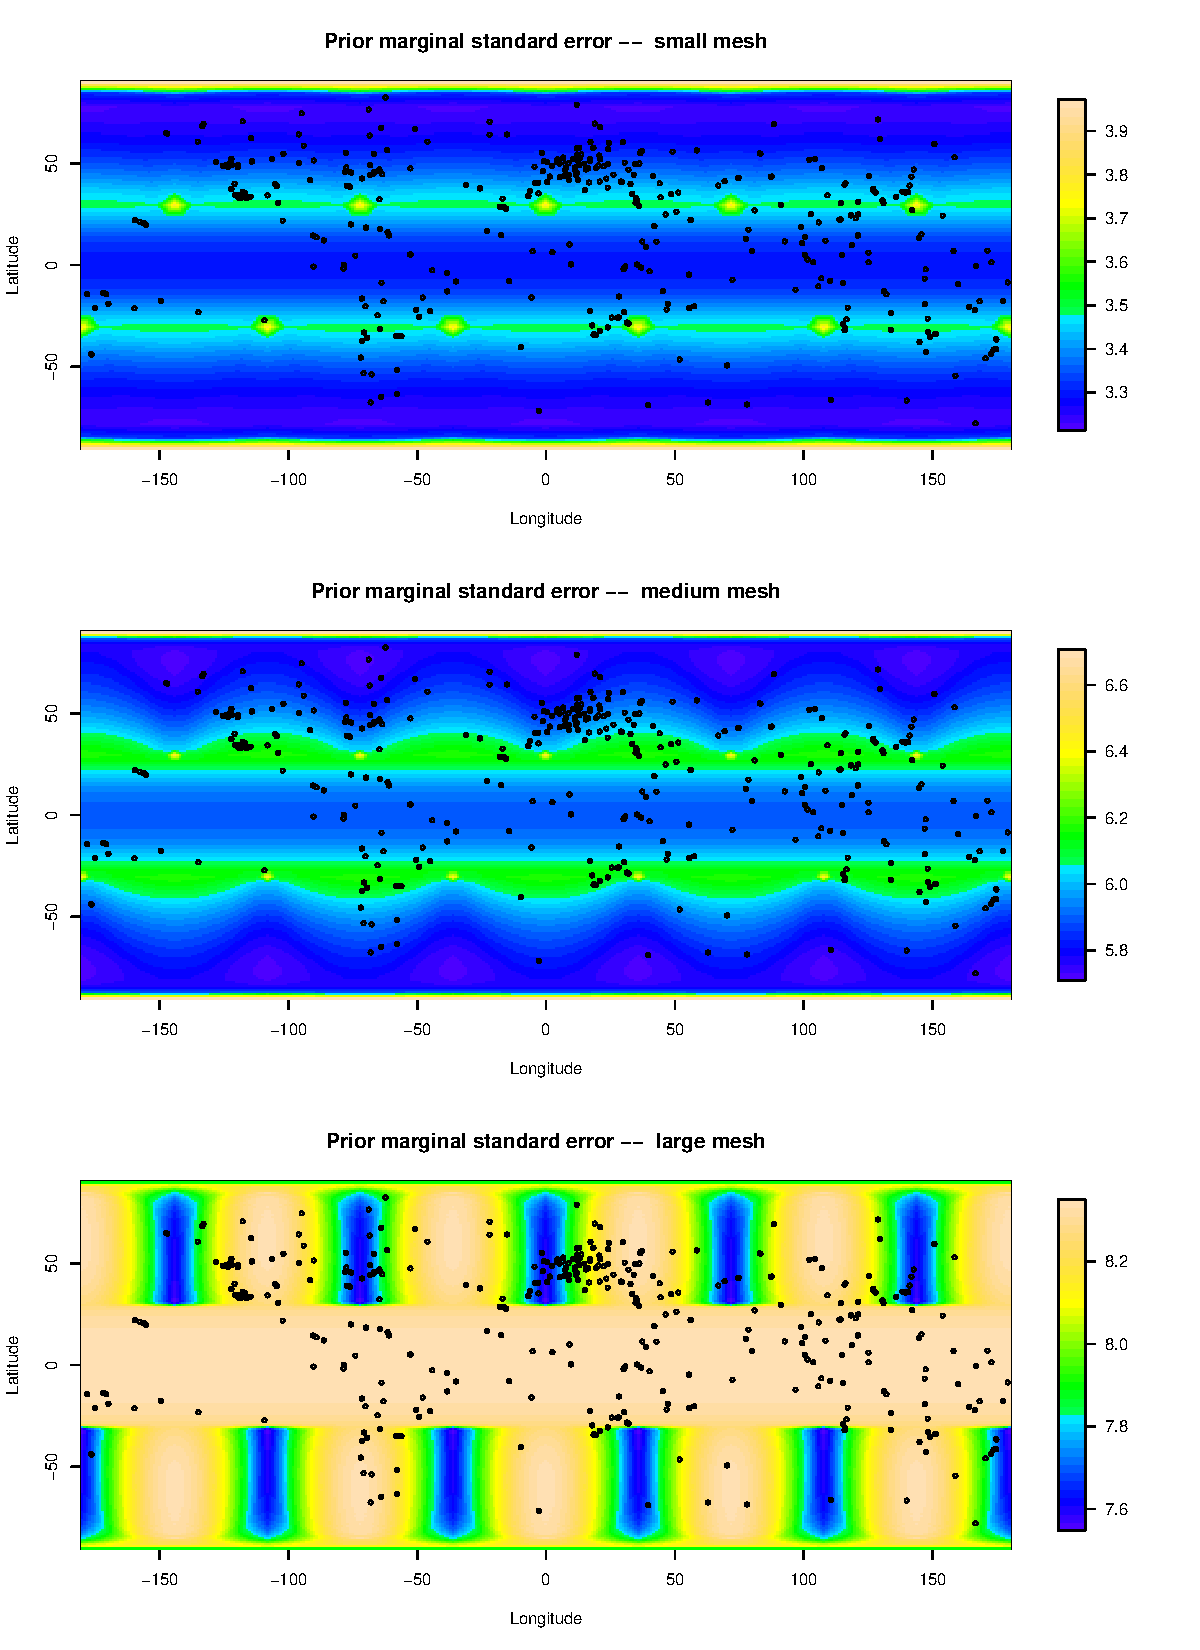
\includegraphics[scale=0.8]{fig/prior_Globemesh.pdf}
 \end{center}
 \caption[Semi-regular mesh]{Marginal standard deviations of the latent field given by semi-regular meshes. The mesh get denser from top to bottom.}
 \label{fig:reg_mesh}
 \end{figure}
Figure \ref{fig:reg_mesh} shows that except a few regular wiggles patterns, the standard deviations are relatively homogeneous. The semi-regular mesh turns out to be the best choice for this experiment.

Future work would be finding better sets of locations to generate a more informative and yet regular mesh. This can be done by patching segmentations and tuning the parameters.
 
\subsection{Comparing estimation and prediction}
In this section, we compare the estimation and prediction results from using different meshes. Based on previous comparison, we choose to use the semi-regular mesh and the large mesh generated by GPS locations in the next experiment and all the followings. We first use INLA to produce fast approximations to the estimation of the hyper parameters and the prediction of the latent field.


\begin{figure}[htbp]
 \begin{center}
 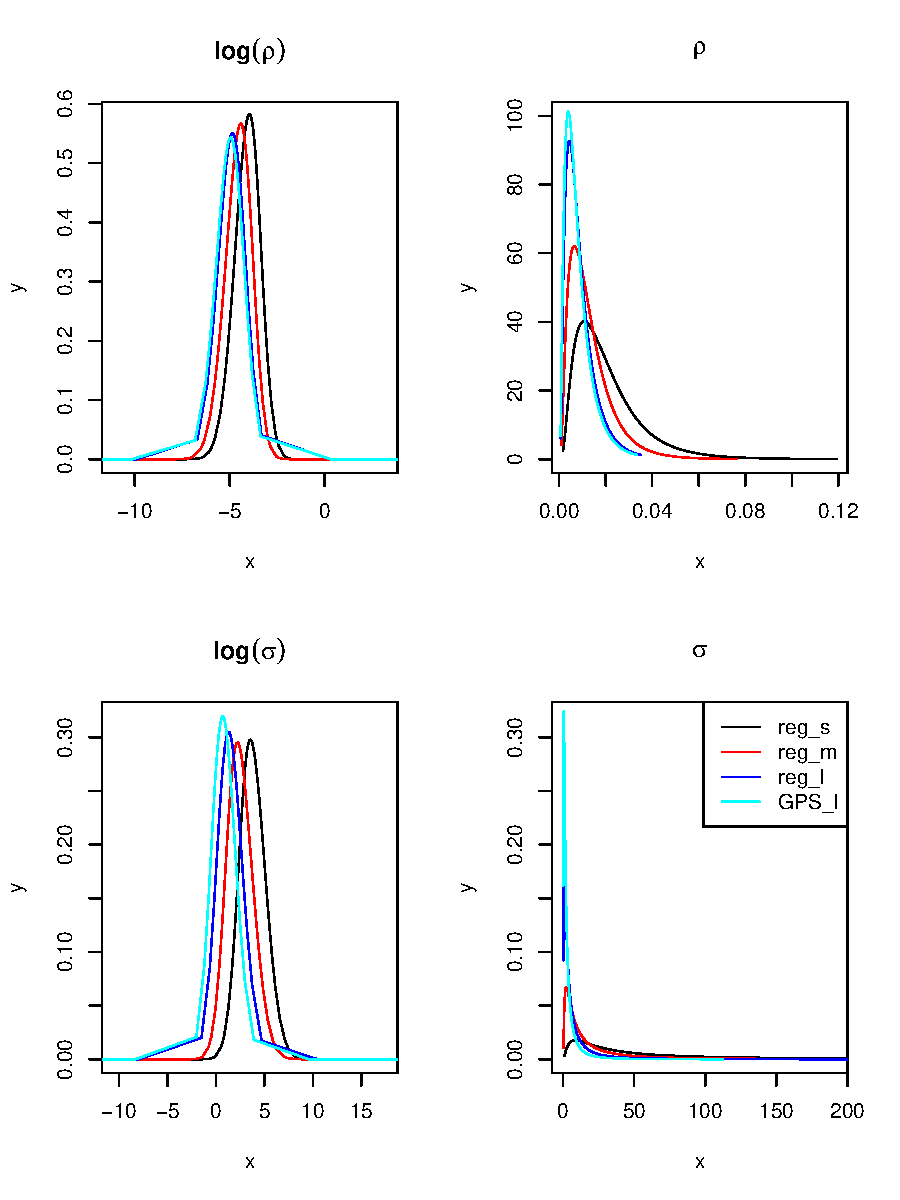
\includegraphics[scale=0.8]{fig/Meshcompare_hyperpar.pdf}
 \end{center}
 \caption[Semi-regular mesh]{Marginal standard deviations of the latent field given by semi-regular meshes. The mesh get denser from top to bottom.}
 \label{fig:mesh_comp_hyper}
 \end{figure}

\begin{figure}[htbp]
 \begin{center}
 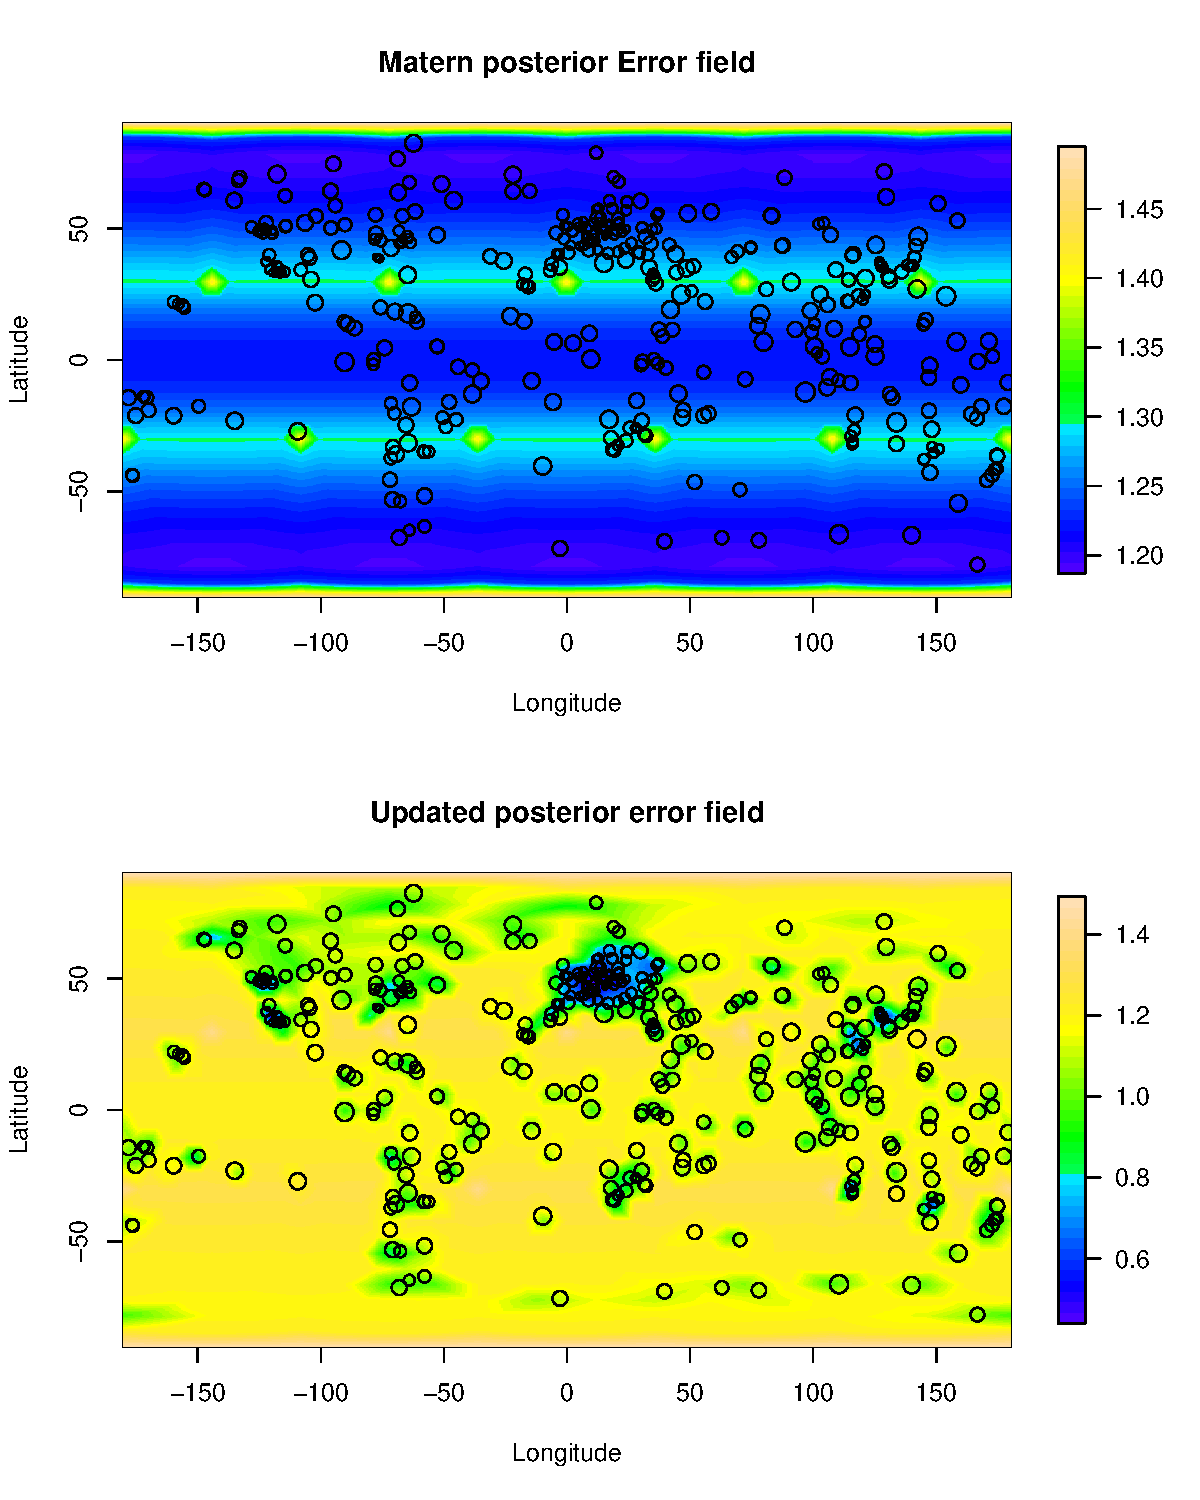
\includegraphics[scale=0.8]{fig/reg_sMeshGIA_error_field.pdf}
 \end{center}
 \caption[Semi-regular mesh]{Marginal standard deviations of the latent field given by semi-regular meshes. The mesh get denser from top to bottom.}
 \label{fig:mesh_comp_hyper}
 \end{figure}

\begin{figure}[htbp]
 \begin{center}
 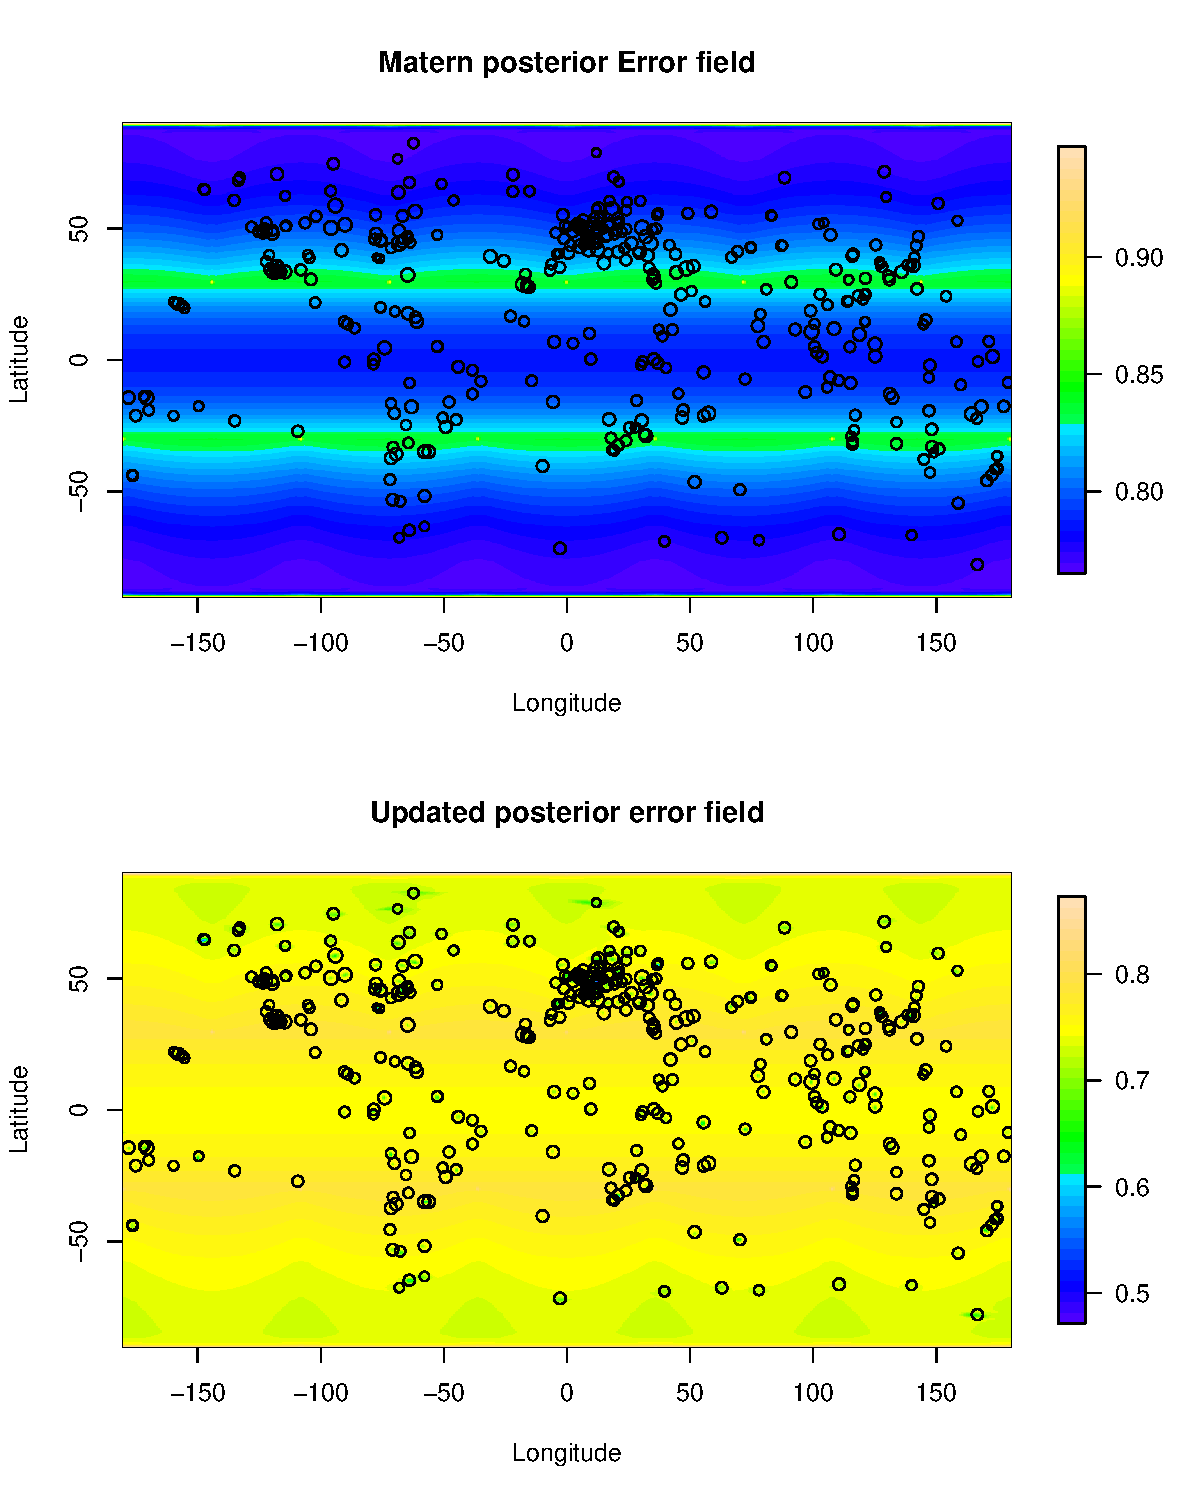
\includegraphics[scale=0.8]{fig/reg_lMeshGIA_error_field.pdf}
 \end{center}
 \caption[Semi-regular mesh]{Marginal standard deviations of the latent field given by semi-regular meshes. The mesh get denser from top to bottom.}
 \label{fig:mesh_comp_hyper}
 \end{figure}

\begin{figure}[htbp]
 \begin{center}
 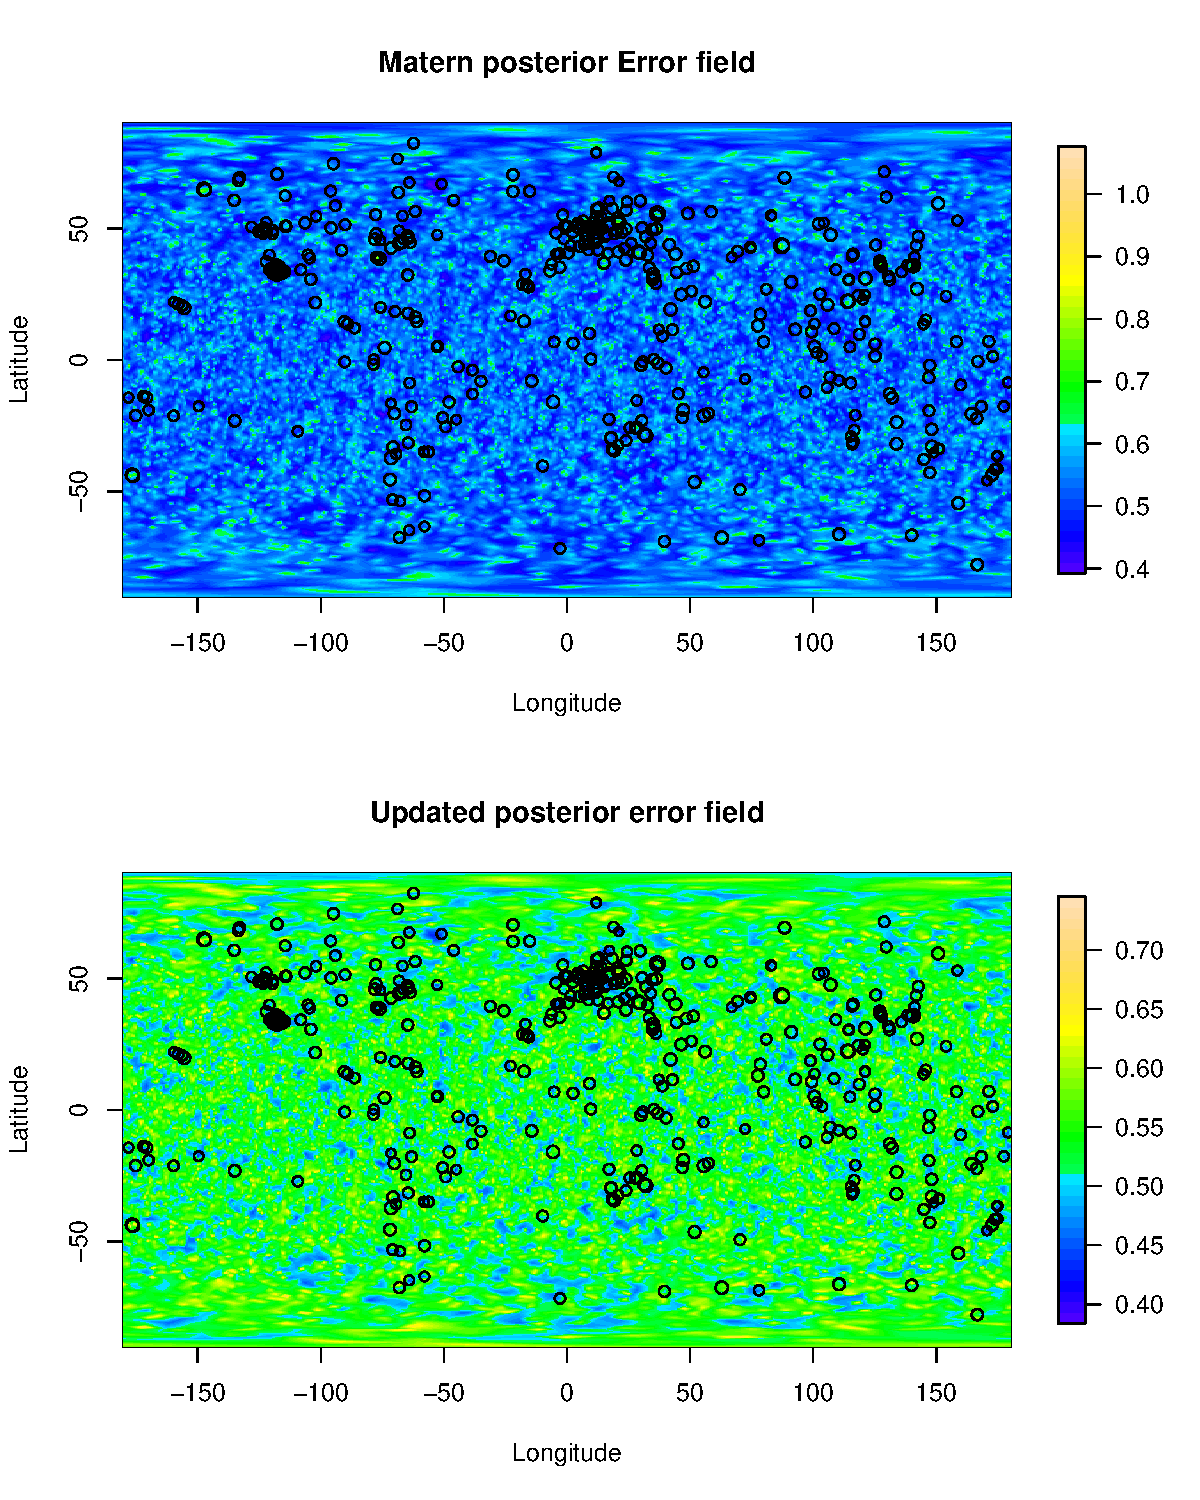
\includegraphics[scale=0.8]{fig/irreg_lMeshGIA_error_field.pdf}
 \end{center}
 \caption[Semi-regular mesh]{Marginal standard deviations of the latent field given by semi-regular meshes. The mesh get denser from top to bottom.}
 \label{fig:mesh_comp_hyper}
 \end{figure}
 
\section{Priors for the hyper parameters}\label{sec:hyperpar}
2. Transformation of the hyper parameter and choosing the prior

\newpage
\section{Test error size}
3. Test the "Principle of stable inference" theorem 
\subsection{Change error size of a single point}
 Compare the effect of error size using a single isolated point.
 
 \begin{figure}[htbp]
 \begin{center}
 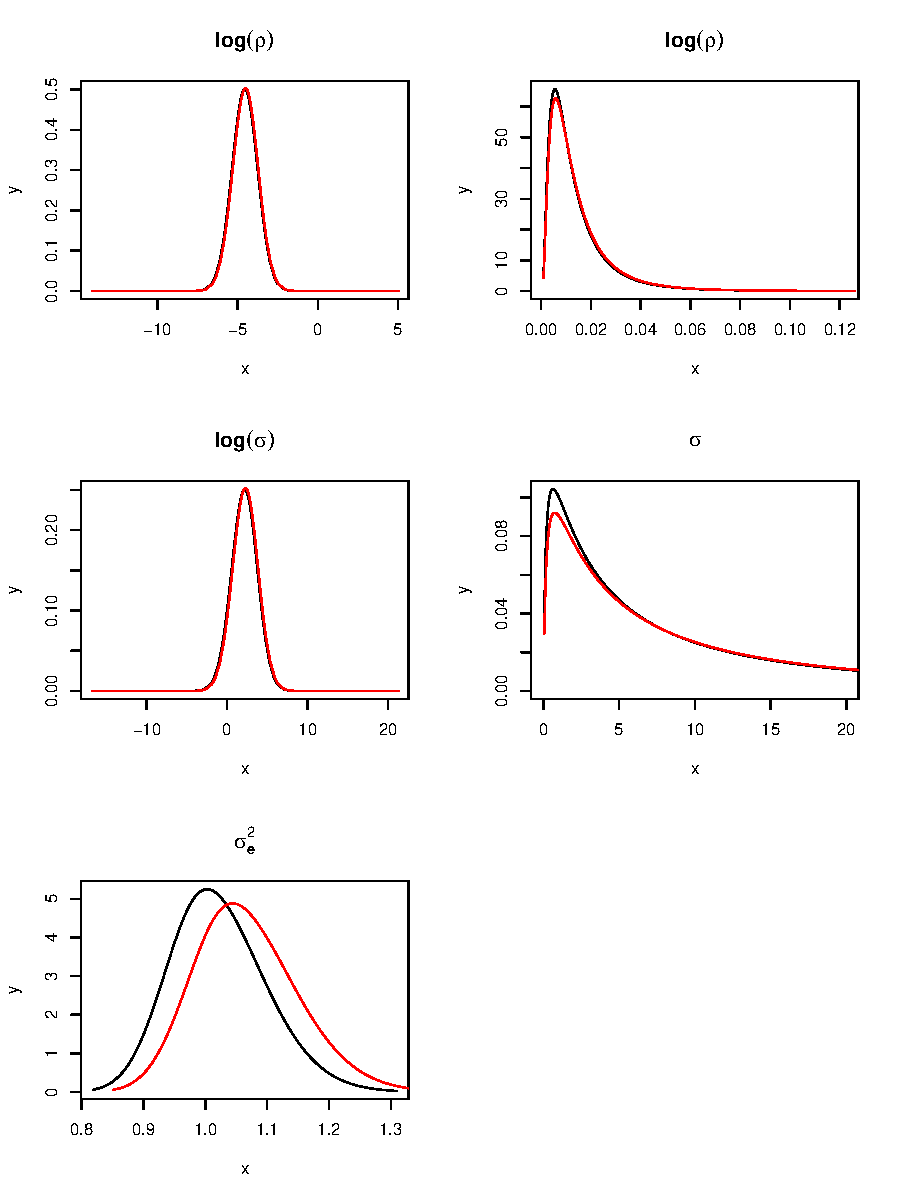
\includegraphics[scale=0.8]{fig/PointErr_hyperpar.pdf}
 \end{center}
 \caption[Posteriors of hyper parameters]{Posteriors of the hyper parameters using different error size for a selected point. Black: small error, Red: large error.}
 \label{fig:5}
 \end{figure}
 
 \begin{figure}[htbp]
 \begin{center}
 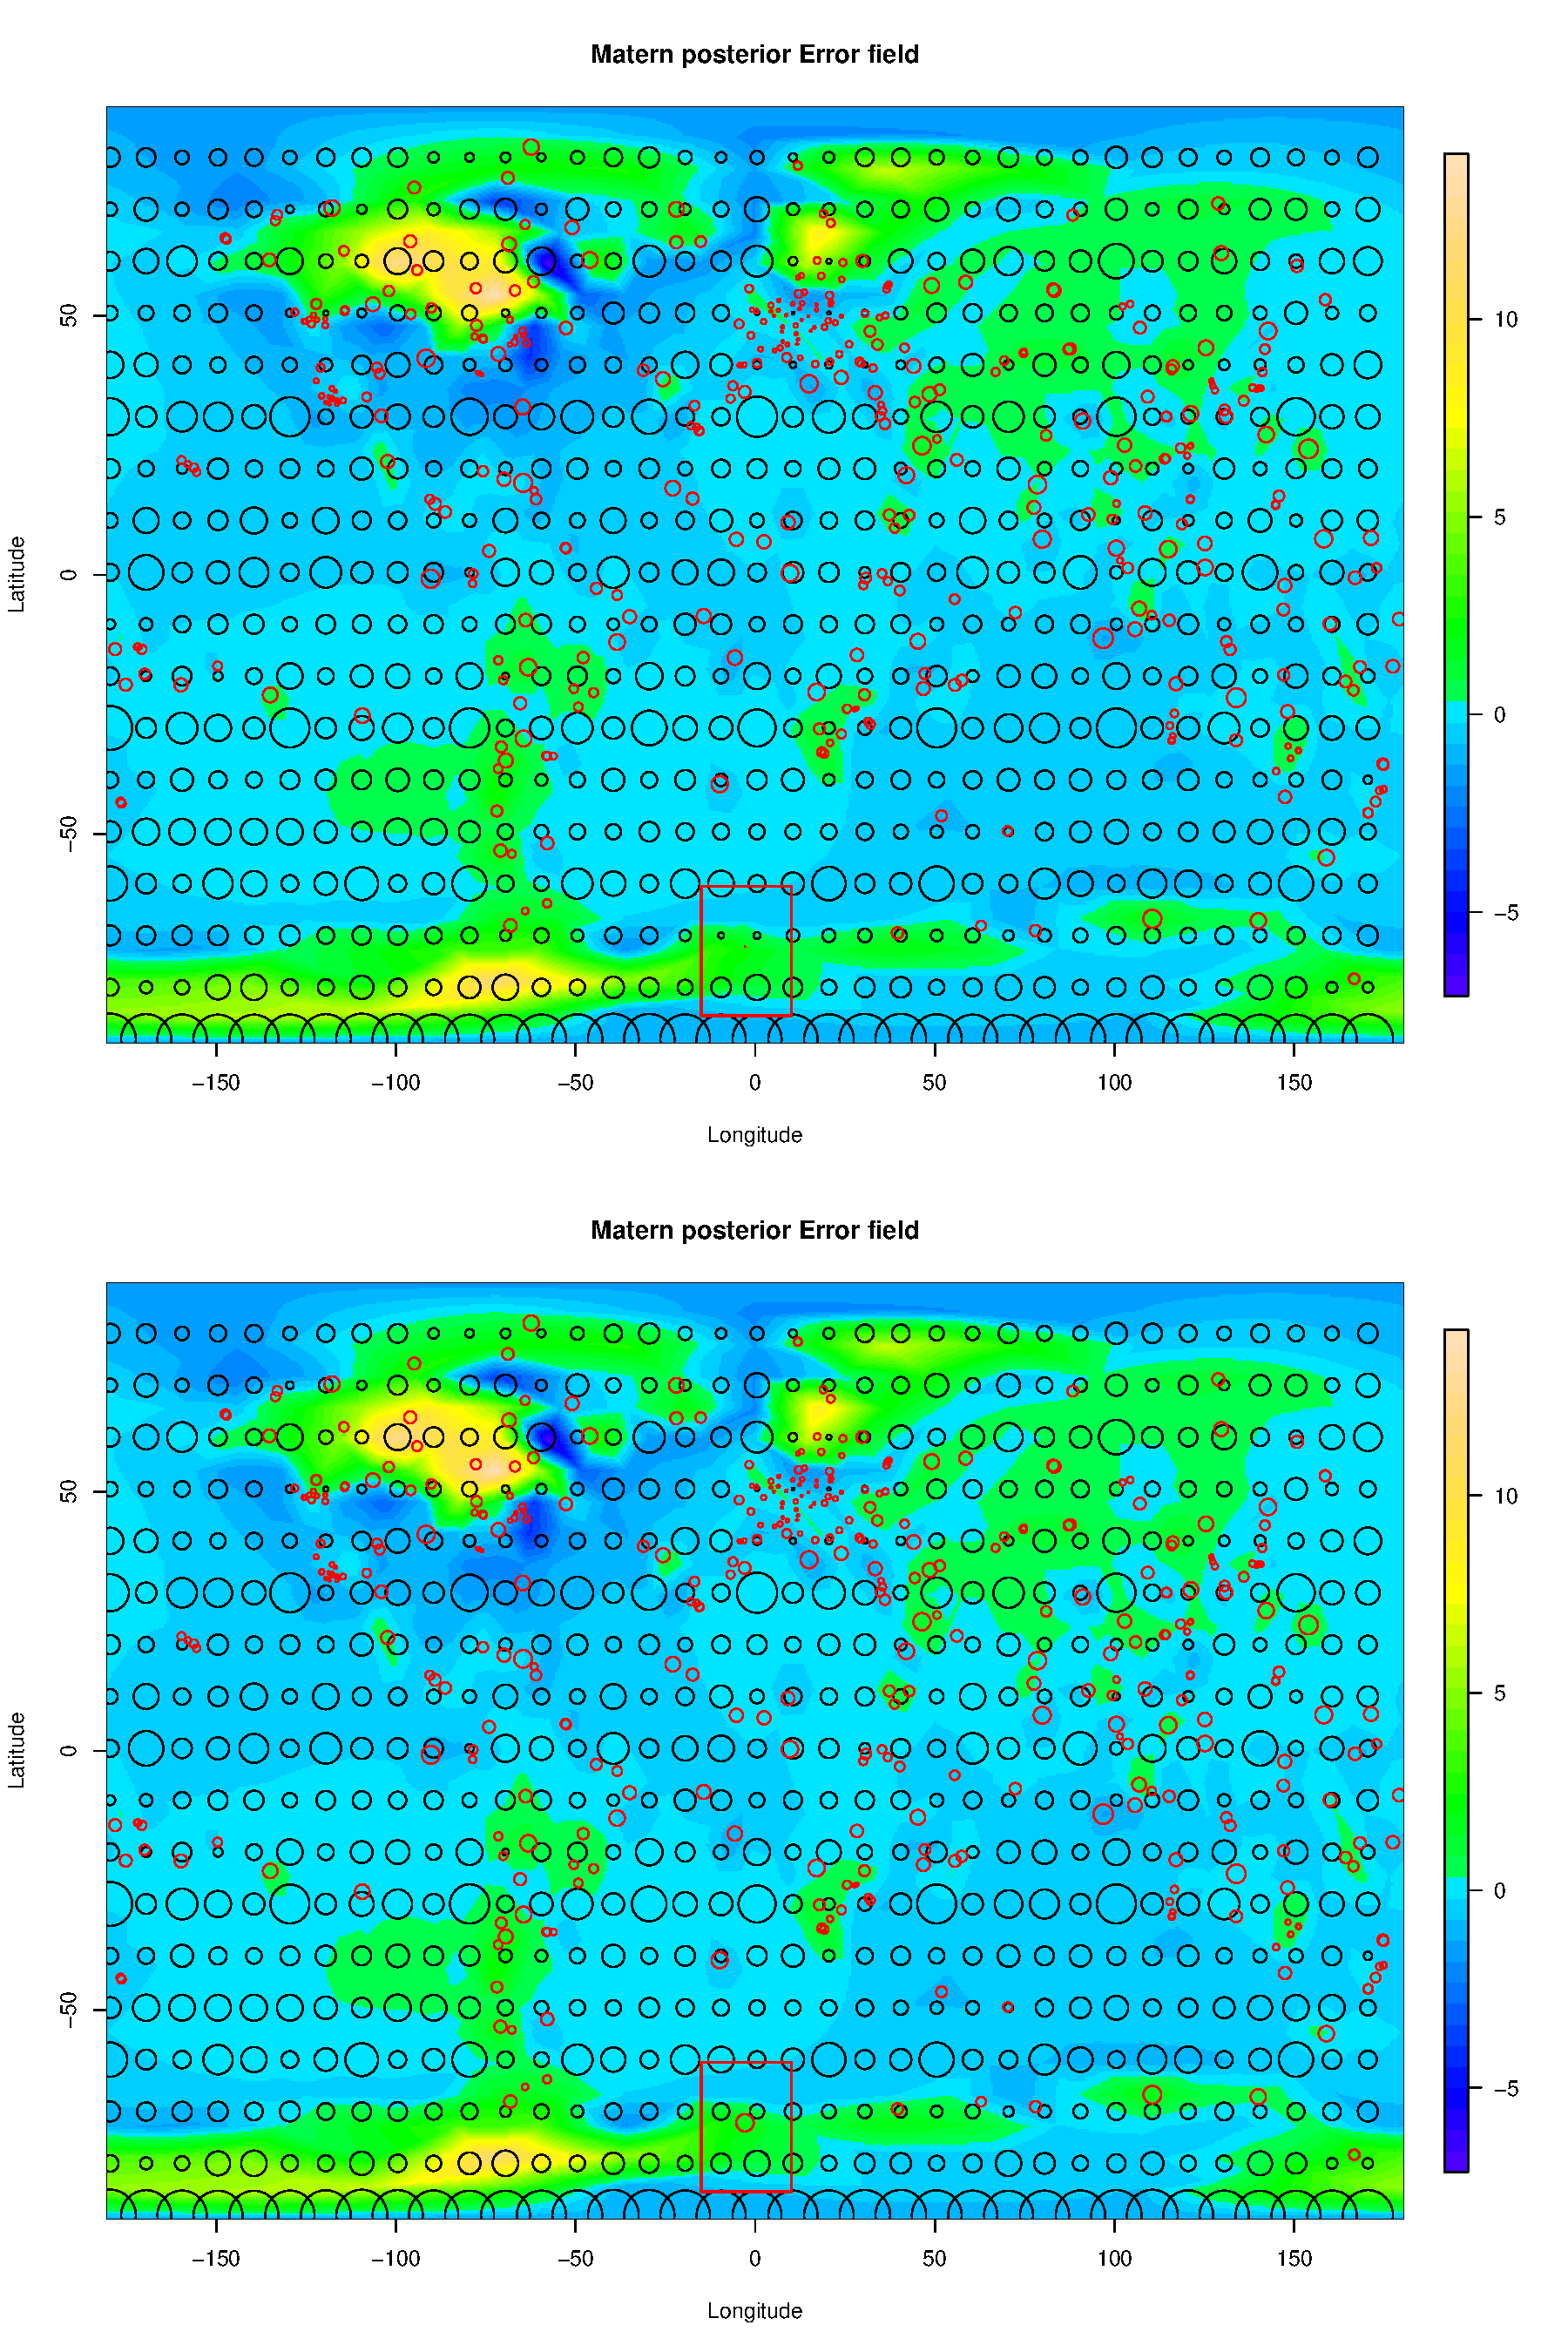
\includegraphics[scale=0.5]{fig/PointErr_GIAfield.pdf}
 \end{center}
 \caption[Posterior marginal standard errors of the latent field]{Posteriors marginal standard errors of the latent field using GPS data with different error on a single selected point. The selected point is marked as the circle within the red rectangle. Points are the GPS locations. Red points are positive errors and black negative. The circle size in the bottom plot represents the error size.}
 \label{fig:6}
 \end{figure}
 
 

\section{MCMC results}

All tested on the smallest mesh grid and use univariate slice sampler for updating the SPDE parameters.





\section{Experiment 1b}


\begin{figure}[htbp]
 \begin{center}
 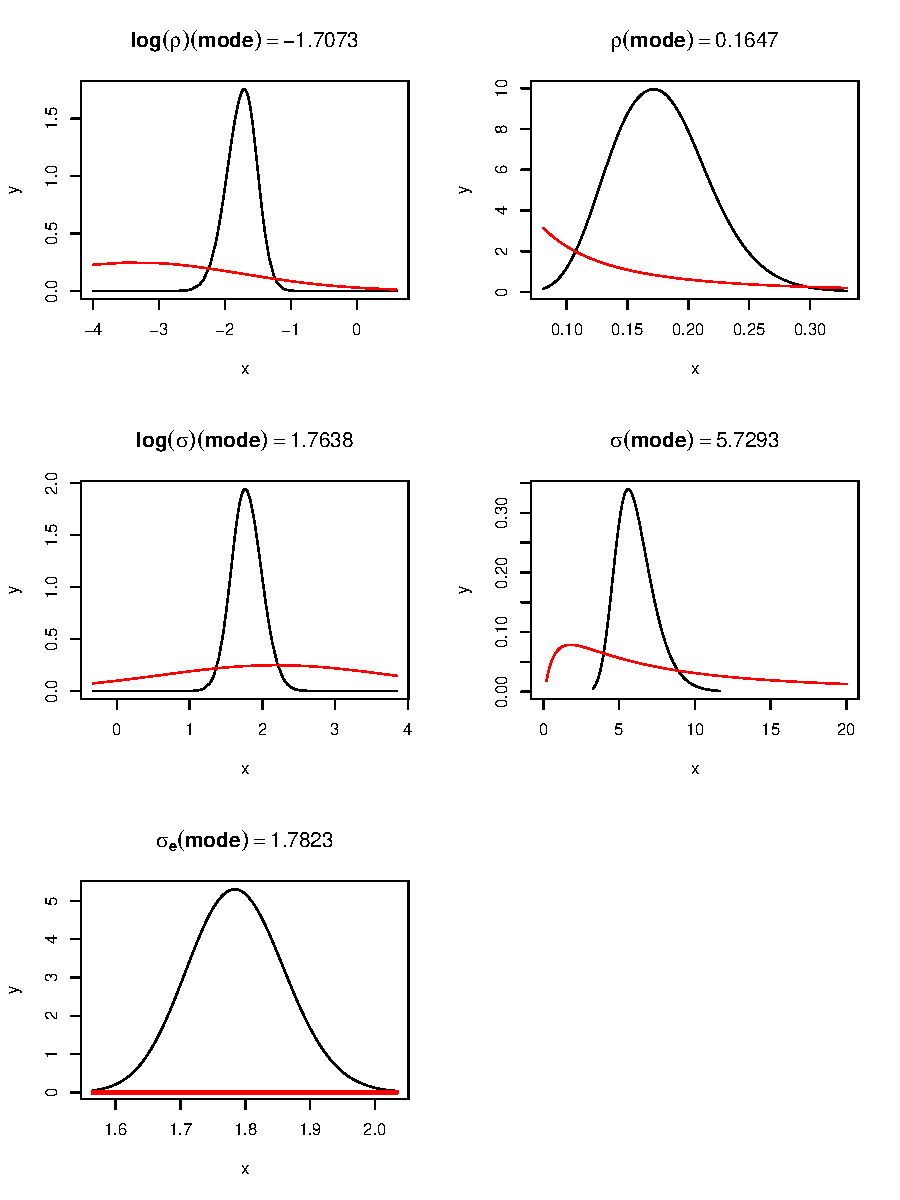
\includegraphics[scale=0.8]{fig/1bsMesh_hyperpar.pdf}
 \end{center}
 \caption[Posterior hyper parameters]{Posteriors of the hyper parameters using INLA.}
 \label{fig:5}
 \end{figure}


\begin{figure}[htbp]
 \begin{center}
 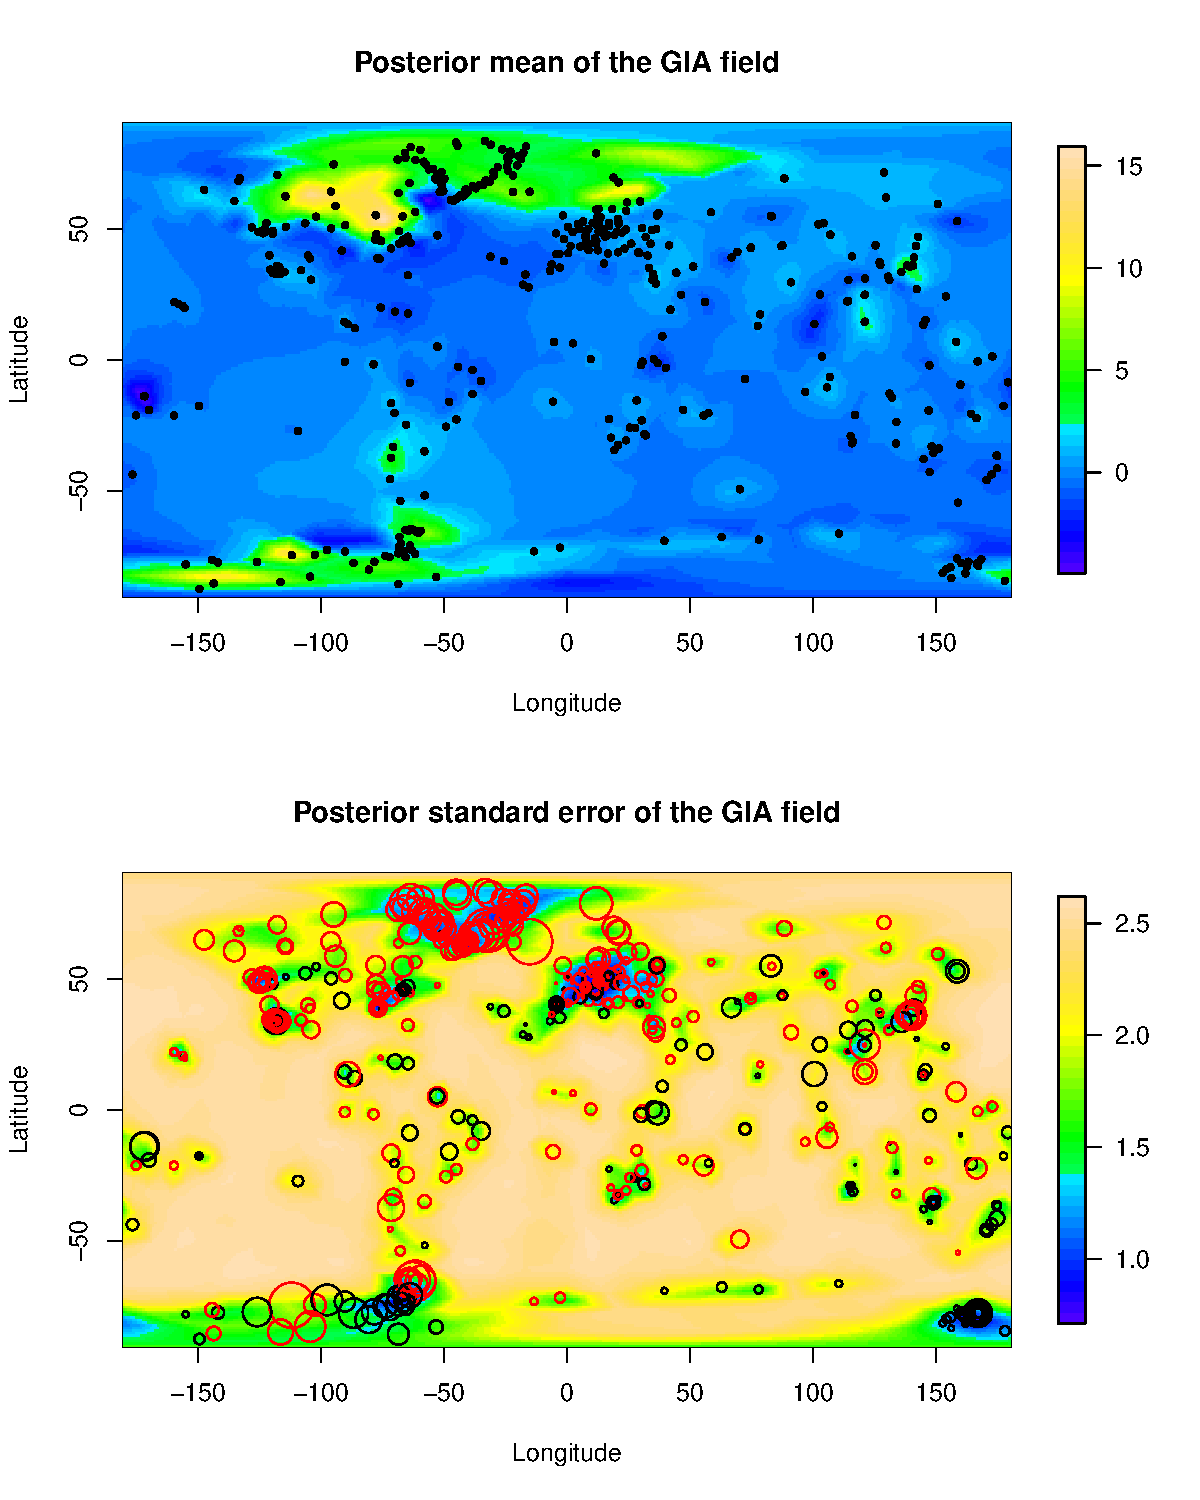
\includegraphics[scale=0.8]{fig/1bsMesh_GIAfield.pdf}
 \end{center}
 \caption[Posterior field]{Posteriors GIA field using INLA.}
 \label{fig:5}
 \end{figure}
 
 \begin{figure}[htbp]
 \begin{center}
 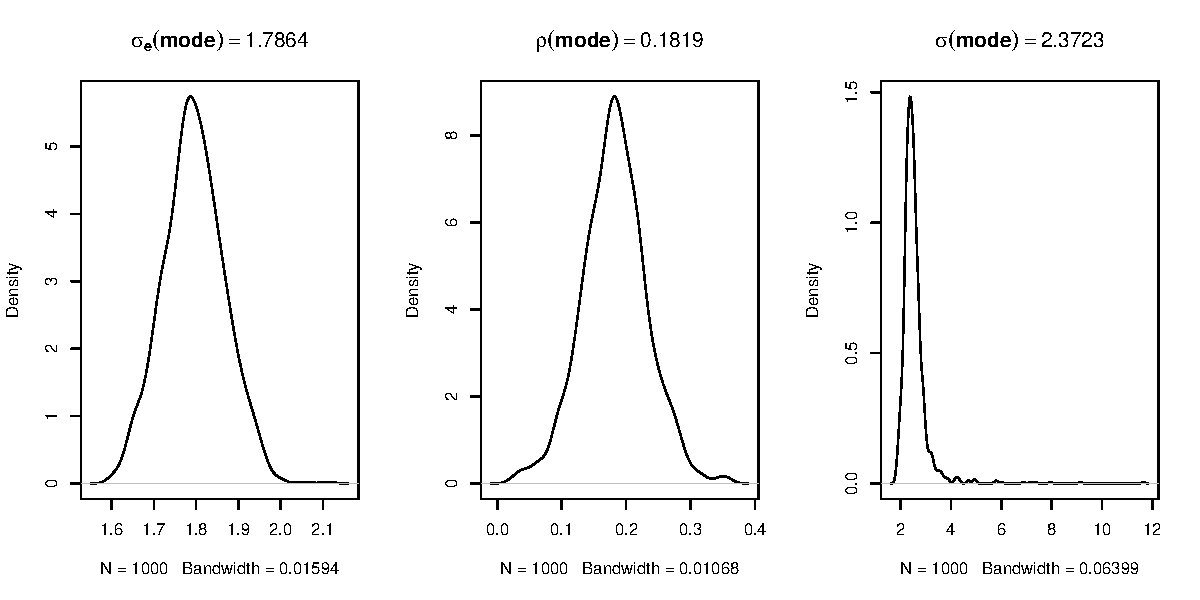
\includegraphics[scale=0.8]{fig/1bslice1_1000_hyperpars.pdf}
 \end{center}
 \caption[Posterior hyper parameters]{Posteriors of the hyper parameters using MCMC.}
 \label{fig:5}
 \end{figure}
 
 \begin{figure}[htbp]
 \begin{center}
 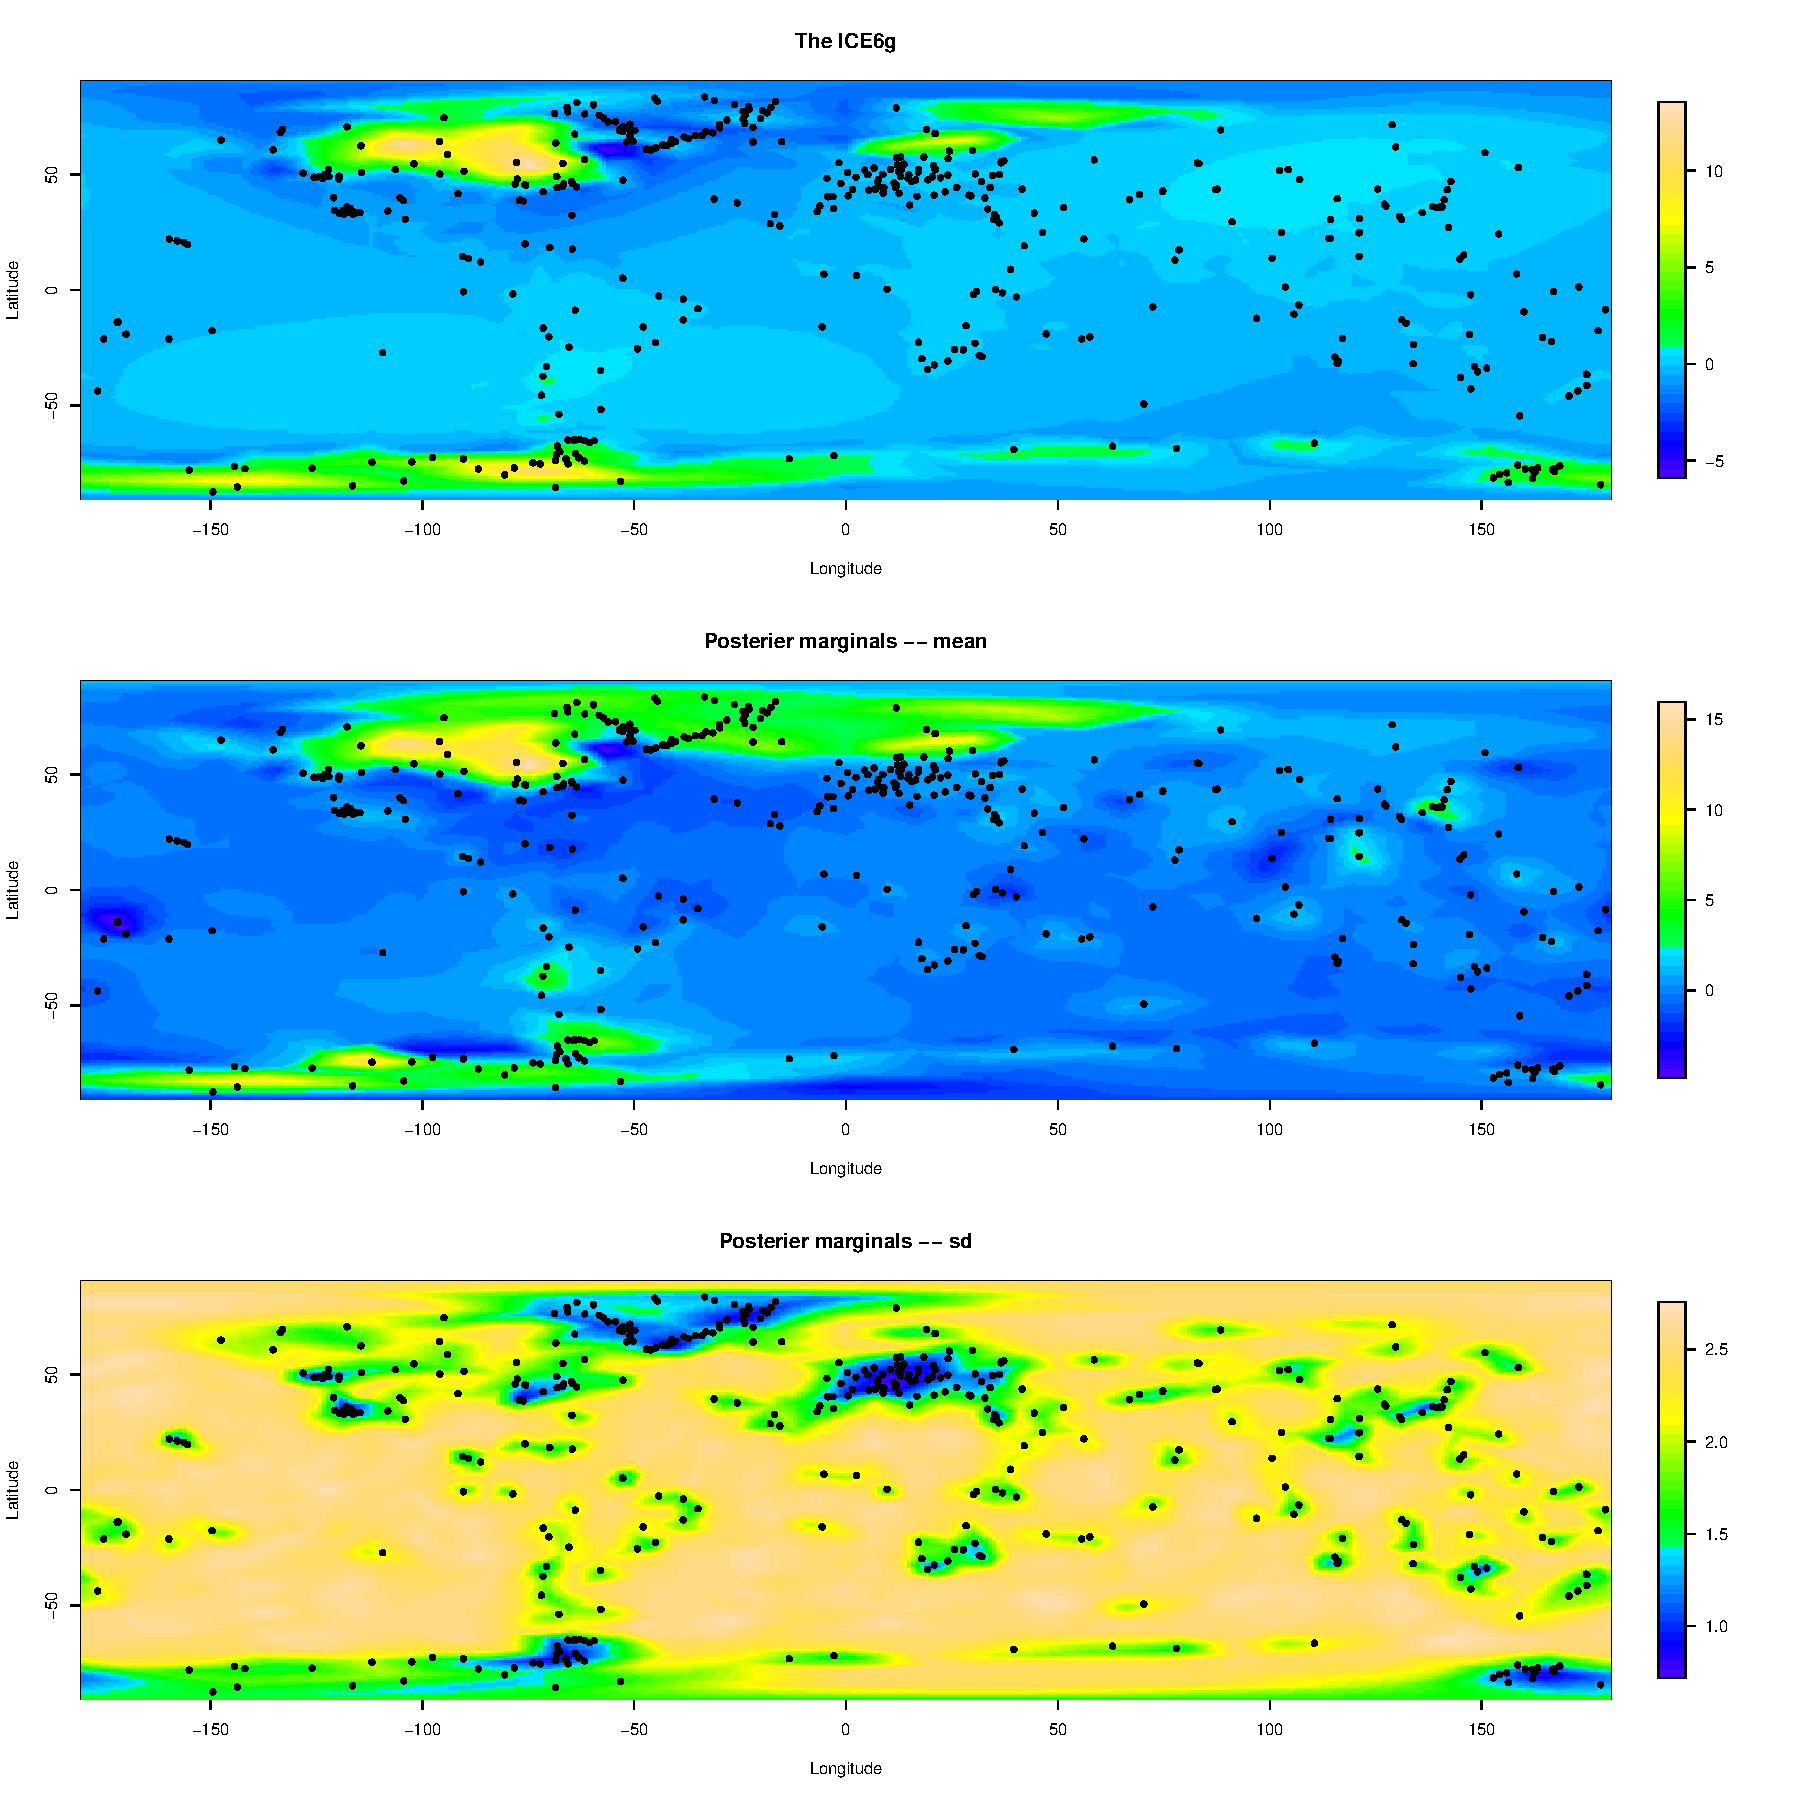
\includegraphics[scale=0.55]{fig/1bslice1_1000_GIAfield1.pdf}
 \end{center}
 \caption[Posterior field]{Posteriors GIA field using MCMC.}
 \label{fig:5}
 \end{figure}
 
 
 

%------------Y(^_^) I'm the happy separation line (^_^)Y-------------%
\bibliographystyle{abbrvnat}
%\bibliography{references}




\end{document}